\documentclass[color=usenames,dvipsnames]{beamer}

\mode<presentation> {

\usetheme{Madrid}
\usecolortheme{lily}
\useoutertheme{infolines}
}
\usepackage{booktabs} 
\usepackage{tikz}
\usepackage{subfigure}
% Thin fonts
\usepackage{cmbright}
\usepackage[T1]{fontenc}

\definecolor{dark_grey}{gray}{0.5}
\setbeamercolor{normal text}{fg=dark_grey,bg=white}
\setbeamertemplate{navigation symbols}{}

\setbeamercolor*{palette primary}{fg=gray!100,bg=gray!10}
\setbeamercolor*{palette quaternary}{fg=gray!100,bg=gray!10}
\setbeamercolor*{palette secondary}{fg=gray!100,bg=gray!20}
\setbeamercolor*{palette tertiary}{fg=gray!100,bg=gray!10}
\setbeamercolor*{navigation symbols}{fg=white,bg=white}
\usefonttheme{default}


\setbeamertemplate{blocks}[rounded][shadow=false]
\setbeamercolor{block title}{bg=gray!10}
\setbeamercolor{block body}{fg=gray,bg=gray!10}
%\setbeamercolor{frametitle}{fg=}

\setbeamertemplate{frametitle}[default][center]

\setbeamertemplate{itemize items}[default]
\setbeamertemplate{enumerate items}[default]


\newcommand{\F}{\mathbb{F}}
\setbeamertemplate{caption}[numbered]

\title{3D-Art Gallery\\ ( Status and Challenges )}
\author[]{Amit Tomar (MT2013008) \\Srinivas Vaidya  (MT2013152)\\ Subarna Sinha  (PH2014009) }

%\vskip .2 cm \fontsize{.3cm}{1em}\selectfont (Under the guidance of Prof. Jaya Sreevalsan Nayar)} 

\institute[IIIT-Bangalore]{International Institute of Information Technology, Bangalore}
\date{Nov 4, 2014}
\begin{document}

\begin{frame}
  \titlepage
\end{frame}

% Uncomment these lines for an automatically generated outline.
%\begin{frame}{Outline}
%  \tableofcontents
%\end{frame}


\section{Standard to be followed}

\begin{frame}{}

\begin{figure}[h!]  
  \centering
  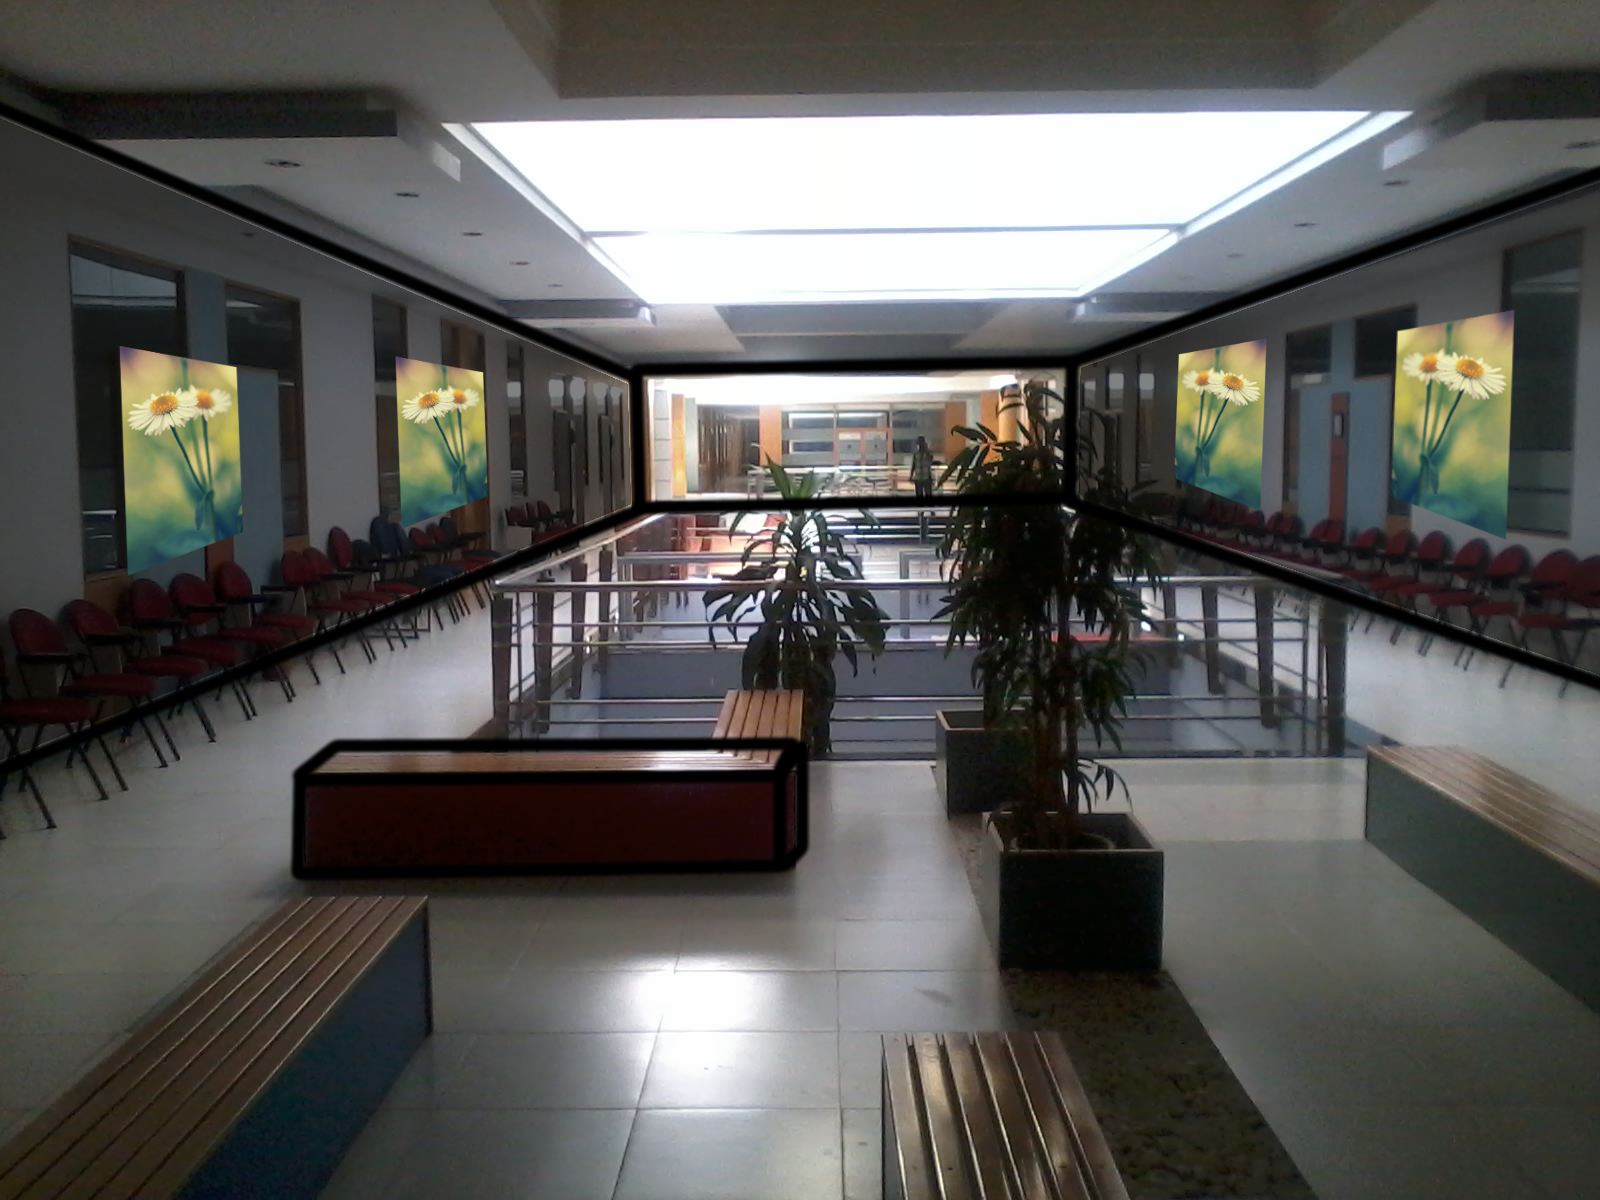
\includegraphics[width=1\textwidth]{3D-ArtGallery.jpg}  
  \end{figure} 
\end{frame}

\section{Introduction}

\begin{frame}{3D-Gallery}

\begin{itemize}

  \setlength{\itemsep}{25pt}
  
\item Gallery modelled as 3-D mesh.

\item Traversal inside the gallery.
  
\item Different viewpoints of the scene - human's and controller's.
  
\item Gallery based on folder hierarchy.

\item How to add the new walls and floor and ceiling?

\end{itemize}
\end{frame}


\section{Introduction}

\begin{frame}{3D-Gallery : Challenges}

\begin{itemize}

  \setlength{\itemsep}{10pt}
  
\item Adding new walls, floor and ceiling would be complicated if we create the walls and put textures completely independently.  

\item One approach : Read wall dimensions from a file and then automatically render the art galllery.
  
\item That would certainly make the gallery easier to modify.

\item Need of a blueprint

\item Need of a text file that would store two pairs of (x,z) coordinates (because in OpenGL the y-direction is considered vertical while x and z represent width and depth).

\end{itemize}

\begin{figure}[h!]  
  \centering
  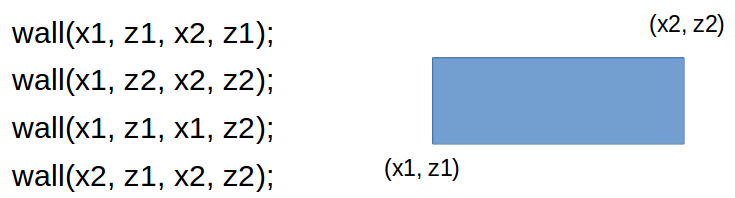
\includegraphics[width=.65\textwidth]{walls.png}  
  \end{figure} 

\end{frame}

\section{Technology}

\begin{frame}{Paintings, Walls, Floors and Lighting}

\begin{itemize}
\setlength{\itemsep}{15pt}  

\item Painting images taken from a folder.
\item Floors, walls and paintings as texture maps.
\item Paintings change on click : 

\begin{itemize}
\setlength{\itemsep}{5pt}  

\item Play movie (Challenge : Performance ?).
\item Deform painting (Challenge : Handling mesh deformation | texture ?).
\item Motion like a pendulum.
\item Falls on floor.

\end{itemize}

\item Lighting in the room and above paintings.
\item Lighting effects (Challenge : Realistic like gallery ?).

\end{itemize}
\end{frame}

\section{Functionality}

\begin{frame}{Human model}

\begin{itemize}

\setlength{\itemsep}{20pt}
  
\item Hierachicaly Modeled (Challenge: Difficult to find parts).
  
\item Can be moved on mouse-click / keyboard.

\item Traverses a path to clicked point.
  
\item Challenges :


\begin{itemize}

\setlength{\itemsep}{12pt}

\vspace {2mm}
  
\item \emph{Realistic} looking motion.  
  
\item Collision detection : Should avoid/jump over obstacles \\(Detection inside the hierarchy or from outside ?).

\item Performance : Multiple models - Kids (Random), Dog (Follows).

\end{itemize}

\end{itemize}
\end{frame}

\section{Standard to be followed}

\begin{frame}{}

\begin{figure}[h!]  
  \centering
  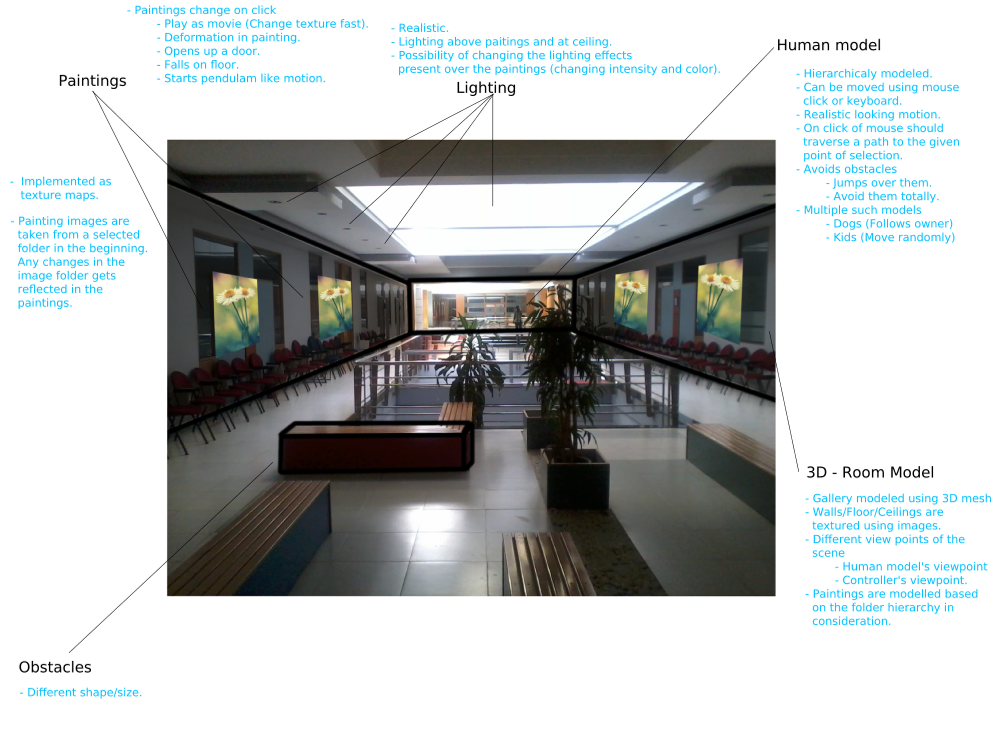
\includegraphics[width=1\textwidth]{3D-ArtGallery.png}  
  \end{figure} 
\end{frame}

\end{document} 